\documentclass[12pt]{report}
\usepackage{graphicx}
\usepackage{float}
\graphicspath{ {images/} }
\usepackage[
backend=bibtex,
style=numeric,
citestyle=numeric,
sorting=none]
{biblatex}
\addbibresource{mybib}
\setlength{\parskip}{5mm}

\begin{document}

\title{OTP and AES: A historical transition between two systems of cryptography}
\author{Valdemar Thanner\\Kantonsschule Zug\\supervised by Mr. Bernhard Keller}
\maketitle

\tableofcontents

\chapter{OTP: The One Time Pad}

\section{What is a "One Time Pad"?}
When speaking about OTP, it is important to distinguish between its two meanings: On the one hand, it is a technique used to encrypt information. This technique requires one single key, used both to encrypt and decrypt the information. This key is also referred to as a one time pad; therefore, it is important to distinguish between the one time pad (a cryptographical technique) and a one time pad (a key which is used to encrypt and decrypt information).

The One Time Pad is largely derived from the Vernam cipher, which is named after Gilbert Vernam. The Vernam cipher utilized a perforated tape (one of the earliest types of data storage) as the secret key\cite{vernampatent}.

\begin{figure}[H]
\centering
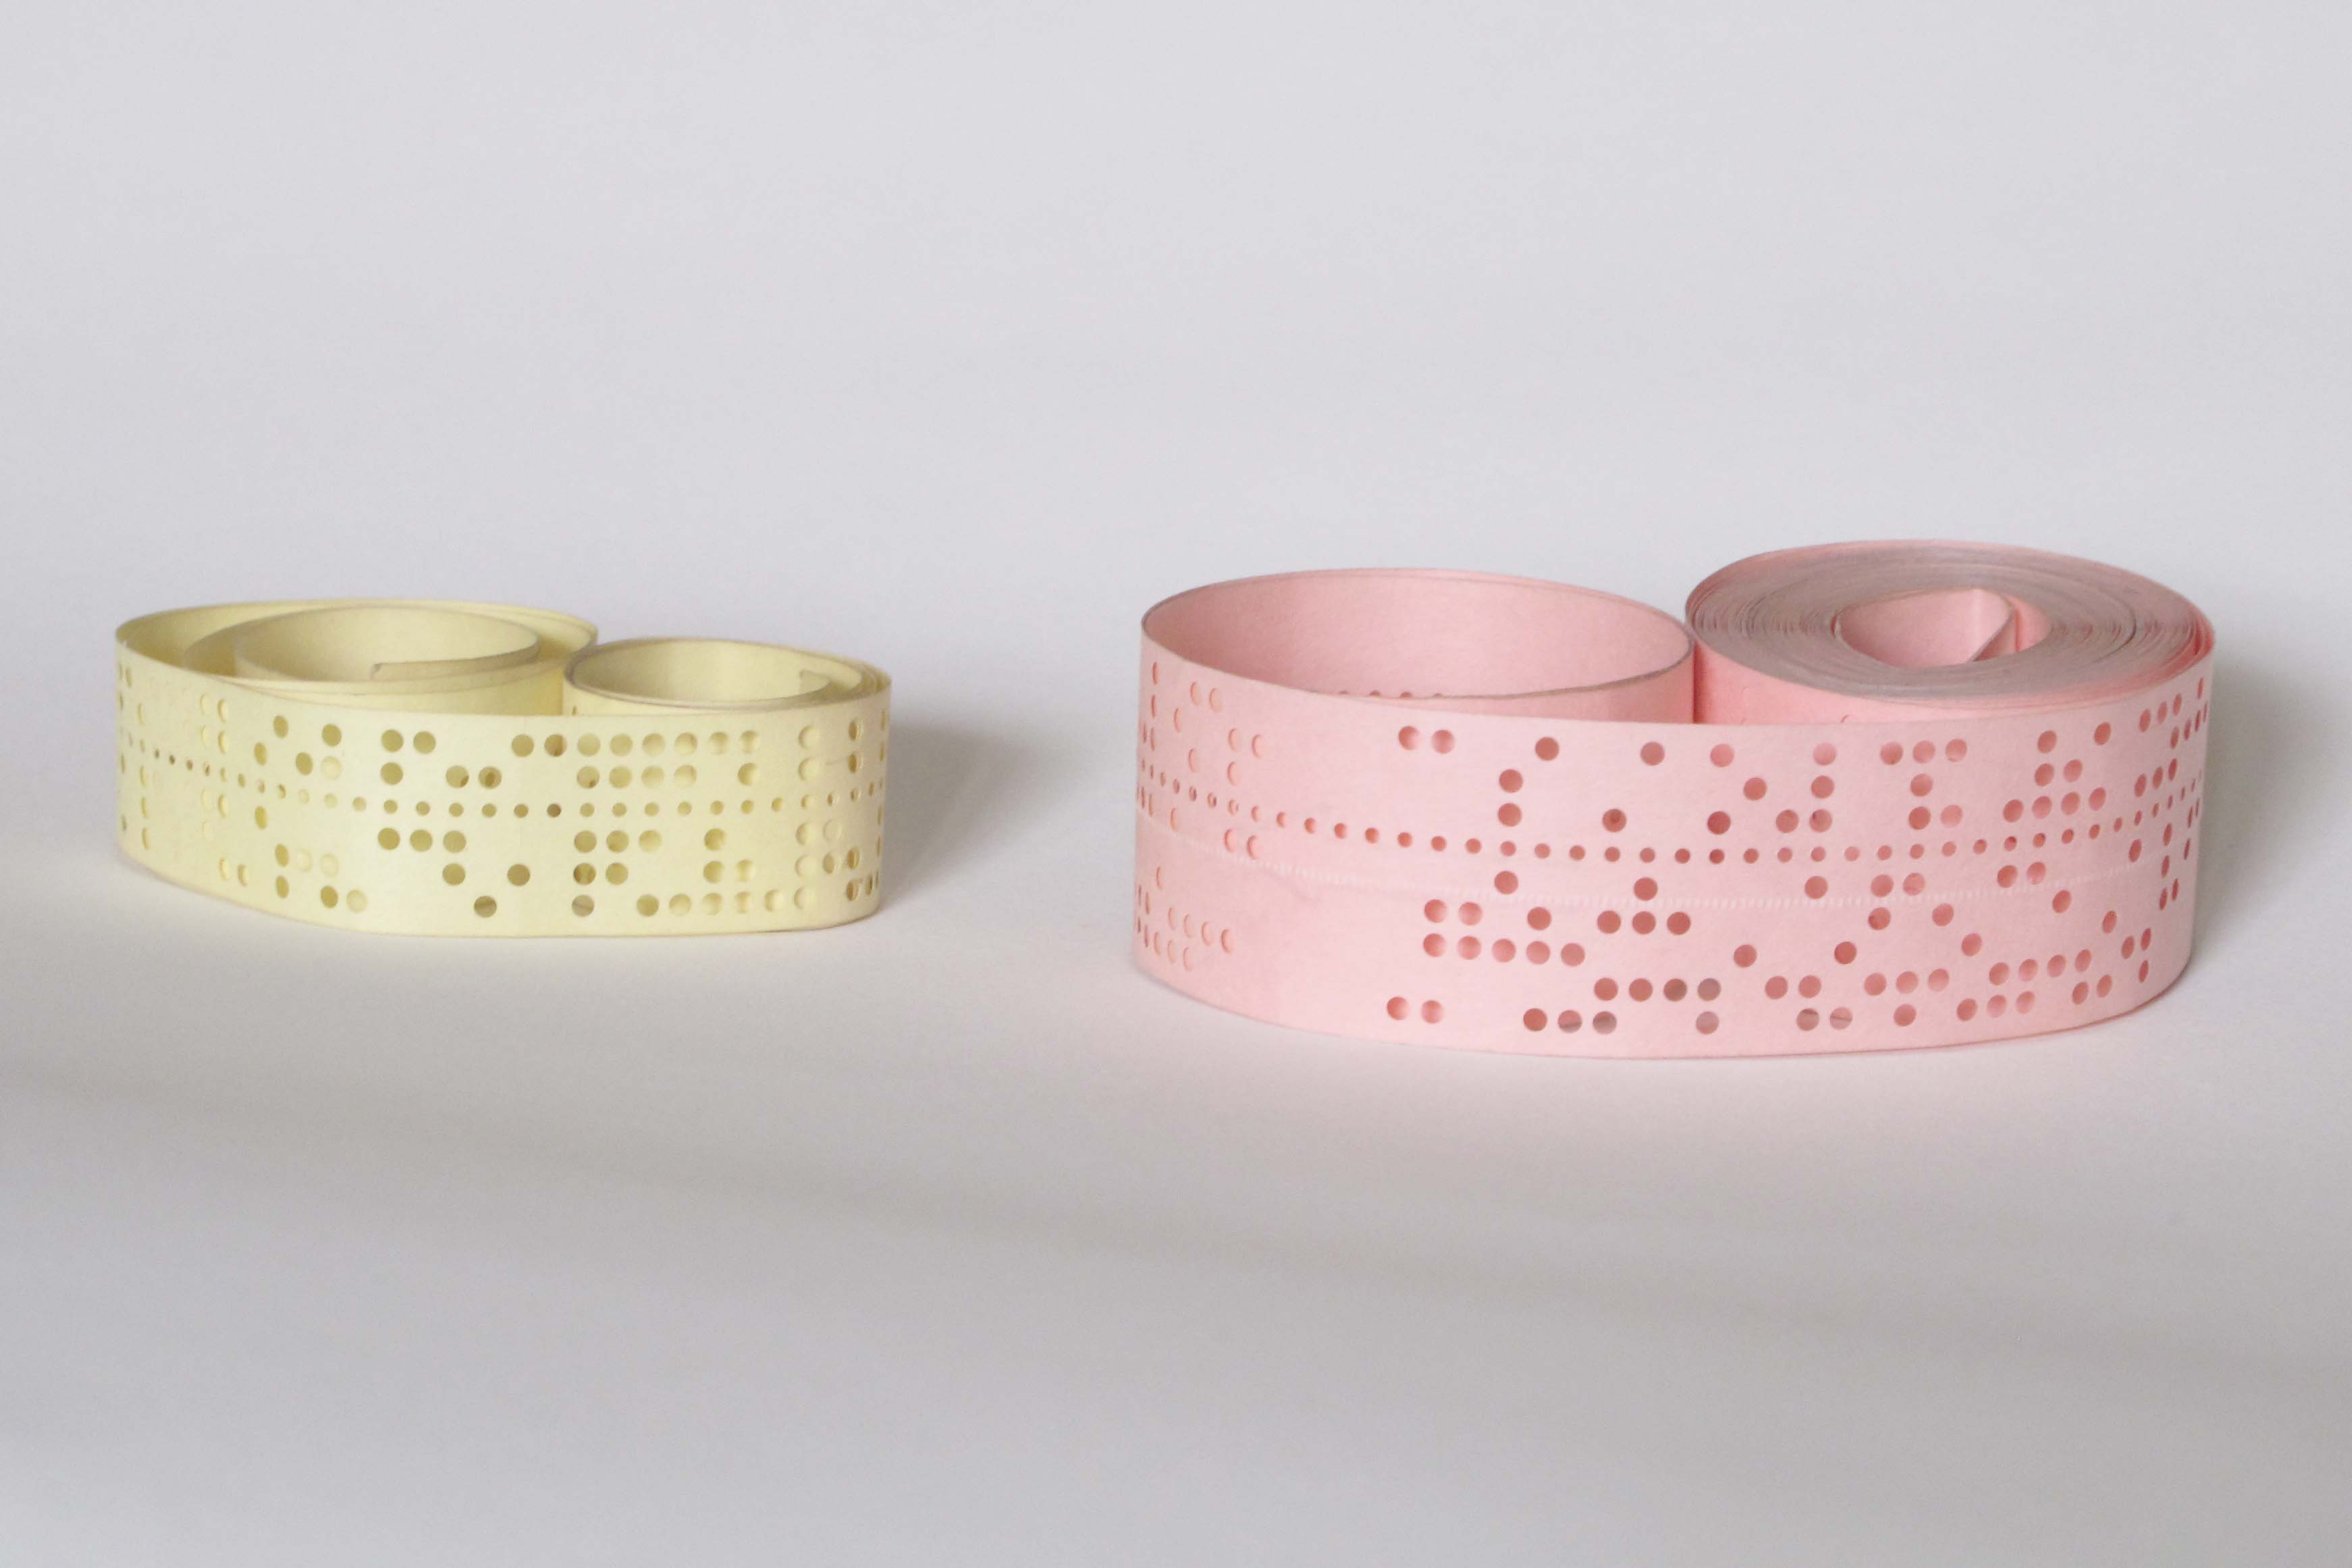
\includegraphics[scale=0.5]{PerforatedTape}
\caption{Perforated tape, utilized to store bits as punched holes}
\end{figure}

However, this system had a vulnerability which the One-Time Pad solved: In Vernam's original method, the perforated tape was not exchanged after it had completed one cycle; instead, it was looped around continuously, often being used multiple times on the same information.    

\section{Method used}
In the following section, the utilized method will be clarified through usage of an example. In this example, the message \textit{"cryptography"} will first be encrypted by it's sender, sent to it's intended recipient, and finally decoded by the recipient.

\subsection{Generation of the random key}
In order to encrypt the plaintext, a key must first be generated. This key will be utilized to encrypt the plaintext through the usage of modular addition, turning it into the ciphertext.

This key must fulfil some crucial criteria. Foremost, the length of the key (the amount of  characters contained within it) must be equivalent to or greater than the length of the plaintext; otherwise, it is not possible to perform any encryption (using the OTP). Secondly, the key must be generated randomly. This is mainly due to the fact that a randomly generated key makes frequency analysis\cite{frequencyanalysis}, the form of cryptanalysis most commonly used to break classical ciphers, impossible.

The key consists of numbers. Usually, when the plaintext is made up of Latin letters, the numbers range between 1 and 26. The key can be converted into Latin letters through the same method applied to the plaintext outlined in the following chapter, however, this is not necessary. 

\subsection{Modular addition of the key and plaintext}
Next, the ciphertext is created through modular addition of the key and the plaintext. This can be applied not only to a message consisting of alphabetical characters, but also to any sequence of bits. If the plaintext consists of a message made up of alphabetical characters, the plaintext and the key are added using arithmetic referred to as \textit{"addition modulo 26"}. 

First, each character (of the plaintext as well as of the secret key, in the case that the key was generated as a string of Latin letters instead of as a sequence of numbers) is assigned a number, corresponding to it's position in the Latin alphabet:

\begin{figure}[H]
\centering
\includegraphics[scale=1]{table1.PNG}
\end{figure}

Afterwards, the key and the plaintext are added together utilizing modular addition. As they are added in modulo 26, this means that any value resulting from the addition which goes above 26 will loop back around:




Finally, the resulting numbers are converted to the character to which they correspond in the latin alphabet. The resulting sequence of characters is referred to as the ciphertext. 

\subsection{decoding of the ciphertext using the key}
Assuming the message has been delivered to the intended recipient, who must hold a copy of the secret key (which, as OTP is a symmetrical cryptographical method, is identical to the one utilized to create the ciphertext), the recipient can now decode the ciphertext in order to view the plaintext.

Since the ciphertext was created through the modular addition of the plaintext and the key, the recipient can utilize modular subtraction in order to view the plaintext. In order to do this, the recipient must subtract the key from the ciphertext in modulo 26.



\section{Perfect secrecy: Information-theoretical security}

\subsection{definition}

%\subsection{mathematical proof}

\subsection{Why can only OTP achieve perfect secrecy?}

\section{Issues with OTP}

\subsection{True randomness in generating the key}

\subsection{Secure distribution of the key itself}

\subsection{Secure disposal of a utilized key}


\printbibliography

\end{document}


